\documentclass[runningheads,deutsch]{llncs}
%
\usepackage[T1]{fontenc}
%
\usepackage{graphicx}
%

% Daniel Motz's packages
\usepackage{amsfonts}
\usepackage{amsmath}
\usepackage{stmaryrd}
\usepackage{amssymb}
\usepackage{mathtools}
\usepackage{ bbold }
\DeclarePairedDelimiter\ceil{\lceil}{\rceil}
\DeclarePairedDelimiter\floor{\lfloor}{\rfloor}

\setcounter{tocdepth}{3}

\usepackage{tikz}
\usepackage{tikz-3dplot}
\usepackage{pgfplots}
\pgfplotsset{compat = newest}

\usepackage{hyperref}

\usepackage{setspace}
\doublespacing

\usepackage{array}   % for \newcolumntype macro
\newcolumntype{C}{>{$}c<{$}} % math-mode version of "l" column type
\newcolumntype{L}{>{$}l<{$}} % math-mode version of "l" column type

\renewcommand{\abstractname}{}
\newcommand{\inline}{\mintinline[fontsize=\normalsize]{c++}{text}}
\newcommand{\estimates}{\overset{\scriptscriptstyle\wedge}{=}}
\DeclareUnicodeCharacter{03BB}{$\lambda$}

\newenvironment{indentleft}[1]{
    \setlength{\leftskip}{#1}
}{
    \setlength{\leftskip}{0pt}
}
\usepackage{cancel}
% END Daniel Motz's packages

\begin{document}
%
\title{
    Einführung in die Künstliche Intelligenz
}
%
\titlerunning{Einführung in die KI}%
\author{Maximilian Stock, Daniel Motz}
%
\authorrunning{M. Stock, D. Motz}
%
\institute{Fakultät für Mathematik und Informatik, Friedrich-Schiller-University,\\ Jena, Germany\\
\vspace{.2cm}
\email{maximilian.stock@uni-jena.de, daniel.motz@uni-jena.de}
}
%
\maketitle % typeset the header of the contribution
%

% Set paragraph indent to 0mm
\parindent0mm
\section{Der Gegenstandsbereich}
%\subsection{Lernfragen}
%\begin{description}
%  \item[Was meint "KI"?] KI ist das Unterfangen, künstliche intelligente Systeme zu bauen. 
%  \item[Der Turing-Test]
%  \item["Starke" und "schwache" KI]
%  \item[Symbolische KI vs. Konnektionismus]
%\end{description}

%\subsection{TODOs}
%\begin{itemize}
%    \item (Seite 10 FS 1) teleologischer Aspekt WB-Systeme verstehen
%    \item (Seite 10 FS 1) "nach generellen Prinzipien strukturiert" verstehen
%    \item (Seite 10 FS 1) Wissenstransfer, Erklärung. Was bedeutet das?
%    \item (Seite 11 FS 1) Wissenstypen: Begriffe abgrenzen
%    \item Hybride (letzte Seite) ergänzen
%\end{itemize} 

%\subsection*{Done TODOs}
%\begin{itemize}
%    \item Den "nicht-einfachen" Turing-Test (die Verhörsituation) verstehen
%    \item Was ist eine einbettende Umgebung in einem PSS?
%    \item PSS genauer definieren
%    \item Starke und Schwache KI nach Searle verstehen
%\end{itemize}

\subsection{Was ist KI?}

\subsubsection{1. Definitionsversuch}

KI ist das Unterfangen, künstliche intelligente Systeme zu \textit{bauen}.
Mit Intelligenz sind Aufgaben, die Menschen gut bewältigen gemeint. Sie
demonstrieren Intelligenz:

\begin{itemize}
    \item Bilderkennung
    \item Stimmerkennung
    \item Aufstellen vernünftigter Erwartungen (z.B. wenn etwas "John" heißt, erwarten wir, dass es sich nicht um ein Kino oder ein Eis, sondern wahrscheinlich um eine Person; vielleicht noch ein Haustier oder Ähnliches). 
\end{itemize}

Nicht alles, was der Mensch gut tut, ist interessant für die KI. 

Viele Aufgaben, die gemeinhin als schwierig (Intelligenz voraussetzen) gelten, sind zu \textit{speziell}: Das einzig intelligente, was ein Schachprogramm kann,m ist Schachspielen!

\subsubsection{Einfacher Turingtest}
\begin{itemize}
    \item Zwei Räume verbunden durch Fernschreiber
    \begin{itemize}
        \item in einem Raum der \textit{Tester}
        \item im anderen: \textit{Mensch} oder \textit{Maschine}
    \end{itemize}
    \item Tester hat 30 Minuten Zeit über den Fernschreiber herauszufinden, ob es sich um einen Menschen oder eine Maschine handelt.
\end{itemize}

\subsubsection{2. Definitionsversuch}

KI ist das Unterfangen, ein künstliches System zu bauen, das den Turingtest zuverlässig besteht.

\subsubsection{Der Turing-Test}
In einer "Verhörsituation" gibt es drei Personen, die sich gegenseitig nicht sehen und nur schriftlich kommunizieren können. Person A ist männlich, Person B ist weiblich und Person C hat ein beliebiges Geschlecht. Person C leitet das Verhör und soll bestimmen, welche der Personen welches Geschlecht hat. C kann beide mit X und Y ansprechen und muss am Ende A X und B Y oder B X und A Y zuordnen. A hat das Ziel, dass C die Geschlechter falsch bestimmt. Auch hier: Zeitlimit von 30 Minuten.

Nun fragen wir uns: "Was passiert, wenn eine Maschine die Rolle von A übernimmt?" 

\subsubsection{Einwände gegen den Turing-Test:}

Kann die Maschine als Mensch durchgehen, nur weil der Tester schlecht ist? (... z.B. einschläft ...) Man wiederholt den Test mehrfach. Der Test ist sinnfrei, wenn $B$ lügen kann, z.B. vorgibt ein Mann zu sein, weil die "Intelligenz" der Maschine dann irrelevant für den Test ist. Er ist auch sinnfrei, wenn $A$ nicht lügen darf. Man geht explizit davon aus, dass $B$ keine Agenda hat.

\subsubsection{Searle's Einwand}

Der Tester tippt nicht mehr als 10 Zeichen pro Sekunde. Die Maschine muss maximal 18.000 Zeichen beantworten. Da die Anzahl an möglichen Anfragen begrenzt ist, kann man in einer riesigen Tabelle alle möglichen Konfrontationen für diesen Dialog speichern und die Maschine kann mit ihrer Hilfe alle intelligenten Reaktionen nachschlagen. Hier scheiden sich die Geister. Wann ist eine KI eine KI und was muss sie können?


\begin{definition}{Die "starke" KI-Hypothese}

\dots eine \textit{funktionale Definition von Intelligenz} $\Rightarrow$ Turing-Test bestehen.

\end{definition}

\begin{definition}{Die "starke" und die "schwache" KI-Hypothese}

Eine schwache KI ist ein Werkzeug, das genau eine Klasse von Problemen lösen kann; zum Beispiel ein Schachcomputer. Für andere Probleme, etwa das steuern eines Fahrzeugs, ist er ungeeignet. Während eine schwache KI ihren Job nur anhand ihres Trainings erledigt, versteht eine starke KI ihre Aufgabe, und ist in der Lage eigenständig eine Lösungsstrategie zu entwickeln. Diese Fähigkeit zu argumentieren und zu abstrahieren, verleiht ihr außerdem die Fähigkeit, sich weiterzuentwickeln, sich zu verbessern und sich neue Fähigkeiten anzueignen. Sie ist autonom.

\end{definition}

\subsubsection{Was heißt hier "künstlich"?}

Minimalforderung: künstlich $\Rightarrow$ anorganisch. Bringt uns aber nicht weiter...

Besser: Ein künstliches System ist ein \textit{physical-symbol-system} (PSS) im Sinne von Newell und Simon. Ein PSS ist eine \textit{symbol-manipulierende Einrichtung} (enthält Symbole, die zusammen Symbolstrukturen bilden, welche erschaffen, bearbeitet, kopiert und gelöscht werden können. Beispiele: \textbf{Turingmaschine}, Universalrechner). Es muss in eine externe Umgebung eingebettet sein, damit man sein Verhalten evaluieren kann.

Beispiel Schach: Unser Schachbrett ist die \textit{planning domain}. In dieser domain kann man sich nur über Züge von Figuren, die Positionen auf dem Brett und ob das Spiel gewonnen oder verloren ist unterhalten. Unsere KI repräsentiert ihre Erkenntnisse als Objekte in dieser domain.

%https://en.wikipedia.org/wiki/Blocks_world

\subsubsection{3. Definitionsversuch}

KI ist das Unterfangen, ein PSS zu bauen, das den Turing-Test zuverlässig besteht.
Zusatzanforderung mancher KI-ler: Die von dem PSS manipulierten Symbole sollen Objekten in der eingebetteten Umgebung entsprechen.

\begin{definition}{Annahme des Deklarativismus.}

    Nach der Annahme des Deklarativismus kann ein System, das alle "intelligenten Antworten" in einer Tabelle nachschlägt, nicht intelligent sein.
\end{definition}

\begin{remark}
    Ein neuronales Netz ist keine deklarativistische Teildisziplin. Außer wenn man so viele Neuronen anlegt, dass alle Beispiele "gemerkt" werden können $\Rightarrow$ \textit{overfitting}.
\end{remark}


\begin{remark}{Kann eine KI stark sein, wenn man auf einem Von-Neumann-Rechner ist?}
    Wahrscheinlich nein, weil er deterministisch ist.
\end{remark}

\subsubsection{Modellierungsansatz}

\begin{enumerate}
    \item Algorithmische Theorie (Problemstellung definieren, Beweis der algorithmischen Lösbarkeit)

    \item Repräsentation und Algorithmus (Algorithmus abstrakt entwerfen. Mithilfe eines Modells, z.B. Von-Neumann-Rechner, geeignete Datenstrukturen wählen)

    \item Implementation (Umsetzung in einer Programmiersprache bzw. Maschinenanweisungen, Optimierung)
\end{enumerate}

Kompetenz: 1. und 2.

Performanz: 2. und 3.

\subsubsection{Wissensbasierte Systeme}

Ein wissensbasiertes System kann als eine besondere Art von Programmiersystemen angesehen werden. Die Inferenzmaschine ist dabei ein Berechnungsmechanismus für mit der Wissensbasis gegebene Programme. Durch die Eingabe von Wissen wird die Inferenzmaschine programmiert. Das Wissen wird deklarativ repräsentiert. Es besteht sowohl aus Faktenwissen (ähnlich den Daten in einer herkömmlichen Datenbank) als auch Regelwissen, zum Beispiel in Form von Produktionsregeln (wenn ..., dann ...), die symbolisch vorliegen. 

Quelle: \href{https://de.wikipedia.org/wiki/Wissensbasiertes_System}{Wikipedia: Wissensbasiertes System}

\pagebreak

\begin{itemize}
    \item methodischer Aspekt -- automatische Lösung mit Fachwissen
    \begin{itemize}
        \item können mithilfe der Ableitungsregeln und dem Wissen in der WB schlussfolgern
    \end{itemize}
    \item qualitativer Aspekt -- schwieriges Problem
    \begin{itemize}
        \item WB-Systeme werden in Feldern angewendet, auf denen imperative, algorithmische Lösung schwer realisierbar sind
    \end{itemize}
    \item teleologischer Aspekt -- praktische Bedeutung
    \begin{itemize}
        \item 
    \end{itemize}
\end{itemize}

Ein WB-System benötigt explizit und deklarativ dargestelltes fachgebietsspezifisches Wissen, das nach generellen Prinzipien strukturiert ist und einen generellen Schlussfolgerungsmechanismus.

\subsubsection{Entwurf}
\begin{itemize}
    \item Wissensdarstellung ("Knowledge Representation")
    \item Wissensausnutzung ("Problem Solving")
    \item Wissenserwerb ("Knowledge Acquisition") $\rightarrow$ Erweiterung / Veränderung der WB
    \item Wissenstransfer, Erklärung ("Explanation")
\end{itemize}

\subsubsection{Wissensrepräsentation}
\paragraph{Wissenstypen}

\begin{itemize}
    \item elementare Tatsachen, Schlussweisen
    \item spezielle Fälle, Situationen
    \item bestimmte Vorgehensweisen, Algorithmen
    \item allgemeine Gesetzmäßigkeiten, Alltagswissen
\end{itemize}

\subsubsection{Logik-basierte Repräsentationsformalismen}
\begin{itemize}
    \item Terminologische Logiken, Beispiel: Diagnosesystem für Fahrzeugdefekte. Symptome als Input, Diagnose als Output)
    \item Vererbung (von Eigenschaften)
    \item Nicht-Monotonie (Monotonie bedeutet, dass bei Erweiterung der Wissensbasis alle bisherigen Schlüsse weiterhin gültig sind. Verwendung von Defaults ist bspw. nicht-monoton.)
\end{itemize}

%\subsubsection{Problemlösungstechniken in WB-Systemen}

%\begin{description}
%    \item[Klassifikation] ...
%    \item[Zugriff] ...
%    \item[Synthese] Schließen von neuem Wissen aus der bestehenden WB (und anschließendes Aufnehmen in die WB)
%    \item[Deduktion] Ableitung mithilfe von Ableitungsregel
%    \item[Simulation] ...
%    \item[Zielorientierte Suche] ...
%    \item[Planen als zielorientierte Suche auf Metaebene] 
%    \item[Strukturanalyse] ...
%    \item[Transformation] ...
%\end{description}

\subsubsection{Einsatzbereiche für WB-Systeme}
\begin{itemize}
    \item Interpretation physikalischer Daten (Messungen interpretieren)
    \item Diagnose von Systemzuständen (Fehler im Auto, kranker Patient)
    \item Planung von Handlungen, um Ziele zu erreichen (Marjapussi)
    \item Entwurf und Konstruktion nach Spezifikation 
    \item Unterricht und Training von Kenntnissen und Fähigkeiten (Deep Learning?)
\end{itemize}

\subsection{Wichtige Teilgebiete der KI}

\subsubsection{Klassische (symbolische) KI}

Die klassische KI nutzt zur Problemlösung Repräsentation für Probleme in (menschenlesbaren) Hochsprachen. Sie nutzt logische Programmierung, Produktionsregeln, semantische Netze und \textit{frames}. Aus ihr entstanden Anwendungen wie Expertensysteme (wissensbasierte Systeme) und automatische Beweisprogramme.

\begin{itemize}
    \item Wissensrepräsentation
    \item Heuristische Suchverfahren
    \item Planung
    \item Wahrnehmung
    \item Deduktion
    \item Lernen
    \item Sprach- und Bildverarbeitung
    \item Verarbeitungsmodelle, KI-Programmiersprachen
\end{itemize}

\subsubsection{Konnektionismus (Soft Computing)}

ist ein Teilgebiet der Kybernetik, welches sich mit dem Verhalten vernetzter Systeme basierend auf Zusammenschlüssen von künstlichen Informationsverarbeitungseinheiten beschäftigt. \textbf{Soft Computing} befasst sich mit der approximativen Lösung. \textit{Es ist von numerischen Verfahren zu unterscheiden.}

\begin{description}
    \item[ Neuronale Netze]
    \item[ Genetische Algorithmen ] (In Anlehnung an die Natur: Suche nach Lösungen mit stochastischen Optimierungsverfahren)
    \item[ Fuzzy Logic ] (Verallgemeinerung der zweiwertigen Booleschen Logik - erlaubt bspw. die Beschreibung der Ausprägung einer Eigenschaft)
\end{description}

%\subsubsection{Hybride}

%\begin{itemize}
%    \item 
%\end{itemize}

\section{Logik}


%\textbf{TODOs}
%\begin{itemize}
%    \item Interpretationsbereich klären (Seite 5 lprelim.div)
%\end{itemize}

\subsection{Lernfragen}

\begin{description}
    \item[Logische Programmierung] Besteht aus einer Menge von Axiomen, die als Fakten oder Annahmen zu verstehen sind, aus denen die Anfrage eines Benutzers beantwortet werden soll. 
    \item[Aussagenlogik] Atome (denen ein Wahrheitswert zugeordnet wird) und Junktoren
    \item[Prädikatenlogik] Erweitert um Prädikate (Aussagen mit Leerstellen, wie eine Funktion) und Quantoren ($\exists, \forall$). Bspw. $\forall x \in \text{Menschen}: \text{mutter}(\text{Eva}, x)$
    \item[Klausellogik] Formel in KNF, bei der die Konjunktionen jeweils in Mengenschreibweise zusammengefasst werden. Bspw.: \\
    $((a \lor b) \land (b \lor c) \land (a \lor \lnot d \lor \lnot e) \land d) \estimates \{\{a,b\}, \{b, c\}, \{a, d, e\}, \{d\}\}$
    \item[Aussagenlogische Resolution] Statt eine allgemeine Gültigkeit zu beweisen, leitet es einen Widerspruch für die Negation her    
    \item[Unifikation] Zwei Ausdrücke werden unifiziert, indem ihre Variablen so durch geeignete Terme ersetzt werden, dass die resultierenden Ausdrücke gleich sind.
    \item[Prädikatenlogische Resolution] Zwei Klauseln $K$ und $K'$ werden resolviert, indem man man ein $\phi$ findet, das in $K$ enthalten ist und dessen Negation $\lnot\phi \in K'$. Man bildet dann die Vereinigung $(K \backslash \phi) \cup (K' \backslash \lnot\phi)$ und nennt sie Resolvente.
    \item[Aussagenlogische Resolution] Exakt analog zu prädikatenlogischer Resolution. Man nimmt den Term und seine Negation aus den zu resolvierenden Klauseln und bilden ihre Vereinigung.
    \item[Inferenz] aufbereitetes Wissen, das aufgrund von logischen Schlussfolgerungen gewonnen wurde
\end{description}

\subsection{Logische Programmierung}
\begin{itemize}
    \item Mit Logik lässt sich Wissen formalisieren
    \item Die \textbf{Prädikatenlogik} 1. Stufe (PL1) die bekannteste Logik
    \item Inferenzmechanismen gestatten es, aus "altem" (explizitem) Wissen, "neues" (implizites) Wissen abzuleiten.
\end{itemize}

Die Klausellogik als syntaktische Teilklasse von PL1 ist für das Theorembeweisen von besonderer Wichtigkeiten

Der auf Klausellogik basierende Resolutionskalkül kann aber auch als \textbf{Programmiersprache} verwendet werden.

Logische Programmierung (z.B. in \textbf{Prolog}) basiert auf \textbf{Klausellogik} und dem Standard-Inferenzmechanismus der \textbf{Resolution}. Prolog ist daher ein \textit{Satisfiability Solver}. Statt Prolog ließe sich eine prädikatenlogische Axiomensammlung auch mit einem anderen SAT-Solver lösen -- der Vorteil besteht darin allerdings in der Einfachheit des Backtracking-Algorithmus. Er besitzt ein vom Programmierer reproduzierbares und planbares Verhalten. 

\[
    \text{Annahmen} \xrightarrow[\text{als Inferenzregel}]{\text{Resolution}} \text{Konklusionen}
\]

\subsection{Syntax der Prädikatenlogik}

Induktiver Aufbau prädikatenlogische Ausdrücke mit:

\begin{enumerate}
    \item \textbf{Konstantensymbolen} $a, b, c, \dots$
    \item \textbf{Funktionssymbolen} $f, g, h, \dots$
    \item \textbf{Variablensymbolen} $x, y, z, \dots$
    \item \textbf{Prädikatensymbolen} likes, father, $\dots$
\end{enumerate}

Man unterscheidet zwischen \textit{Termen, Atomformeln}.
Ein \textbf{Term} ist entweder

\begin{itemize}
    \item ein Konstantensymbol,
    \item ein Variablensymbolen
    \item ein Funktionssymbol angewendet auf ein Tupel (geordnete Anordnung) von Termen.
\end{itemize}

Eine \textbf{Atomformel} ist ein Prädikatsymbol, angewendet auf ein Tupel von Termen.

Ein \textbf{Grundterm/Grundformel} ist ein Term/eine Formel, der/die keine Variablen enthält.

\begin{example}
    $a, x$ und $f(b, f(b, y, z), y)$ sind Terme.\\
    $\text{likes}(x, \text{dad}(x))$ und \\
    $\text{borrows}(\text{doug}, \text{book}, \text{chris})$ sind Atomformeln.
\end{example}

Eine \textbf{wohlgeformte Formel} ist entweder eine Atomformel oder hat eine der folgenden Formen $(W_1, W_2, W \text{ seien wohlgeformt}):$

\begin{align}
    (W) \\
    W_1 \land W_2 \\
    W_1 \rightarrow W_2 \\
    \lnot W \\
    W_1 \lor W_2 \\
    (\exists X) W \\
    (\forall X) W
\end{align}

Der \textbf{Gültigkeitsbereich} einer Quantifikation $\forall x$ (bzw. $\exists x$) in einer Formel $\forall x \text{F}$ (bzw. $\exists x \text{F}$) ist genau die Teilformel F. Die Variable $x$ heißt dann \textbf{gebunden} in $\forall x \text{F}$ (bzw. $\exists x \text{F}$).

Eine Variable, die in keiner Teilformel einer Formel F gebunden auftritt, heißt \textbf{frei} in F.

Eine \textbf{geschlossene Formel} ist eine wohlgeformte Formel, in der jedes Vorkommen eines jeden Variablensymbols gebunden ist.

\begin{example}
    $(\forall x)((\exists y) \text{child}(x) \rightarrow \text{father}(y, x)).$
\end{example}

Bindungsregeln der logischen Konnektoren und Quantoren:

\setlength{\tabcolsep}{12pt}
\begin{center}    
    \begin{tabular}{l l l}
        $\lnot$           & bindet stärker als & $\land$ und $\lor$ \\
        $\land$ und $\lor$ & bindet stärker als & $\rightarrow$
    \end{tabular}
\end{center}

\subsection{Prädikatenlogik -- die Semantik}

Die Bedeutung einer logischen Sprache wird mithilfe einer \textbf{Interpretation $I$} festgelegt:

\begin{enumerate}
    \item Der \textbf{Interpretationsbereich} $D = dom(I)$ ($dom \estimates$ \href{https://en.wikipedia.org/wiki/Domain_of_discourse}{domain of discourse}) ist eine (nichtleere) Menge von Objekten, auf die sich $I$ bezieht.
    \item Jedem Konstantensymbol wird genau ein Element aus $D$ zugeordnet.
    \item Jedem $n$-stelligen Funktionssymbol wird genau eine Funktion von $D^n \mapsto D$ zugeordnet.
    \item Jedem $n$-stelligen Prädikatsymbol wird genau eine $n$-stellige Relation aus $dom(I)^n$ zugeordnet.
\end{enumerate}
Eine Interpretation weist jeder Formel $G$ einen Wahrheitswert zu:
% TODO weist eine Interpretation einer Formel wirklich einen Wahrheitswert zu?

\begin{itemize}
    \item $I \vDash G$, wenn $I$ der Formel $G$ den Wert \textbf{wahr} zuordnet und
    \item $I \nvDash G$, falls $I$ der Formel $G$ den Wert \textbf{falsch} zuordnet.
\end{itemize}

\subsection{Wahrheitswert zusammengesetzter Formeln}

Prinzip der \textbf{Kompositionalität}:

Der Wahrheitswert einer Formel setzt sich aus den Wahrheitswerten ihrer Teilformeln zusammen.

\begin{center}
    \begin{tabular}{l l l l}
        $\lnot W$ & wahr & $\Leftrightarrow$ & $W$ falsch \\
        $W_1 \land W_2$ & wahr & $\Leftrightarrow$ & $W_1$ wahr und $W_2$ wahr \\
        $W_1 \lor W_2$ & wahr & $\Leftrightarrow$ & $W_1$ wahr oder $W_2$ wahr \\
        $W_1 \rightarrow W_2$ & falsch & $\Leftrightarrow$ & $W_1$ wahr und $W_2$ falsch
    \end{tabular}
\end{center}

$(\forall x) W$ ist wahr gdw. für \textbf{jedes} Element $e$ aus $\mathcal{D}$, durch Ersetzen der Variablen $x$ durch $e$ eine wahre Formel entsteht, sonst falsch.

$(\exists x) W$ ist wahr gdw. für \textbf{ein} Element aus $e$ aus $\mathcal{D}$, durch Ersetzen der Variablen $x$ durch $e$ eine wahre Formel entsteht, sonst falsch.

\subsection{Begriffe aus der Modelltheorie}

\subsubsection{Modelltheorie}
Inhalt der Modelltheorie sind die Beziehungen zwischen den rein formalen Ausdrücken einer Sprache (syntaktische Ebene) und deren Bedeutung (semantische Ebene). Diese Beziehung wird über sogenannte Interpretationen und eine als Erfüllungsrelation bezeichnete mathematische Relation hergestellt.

Gibt es für eine Formel $F$ eine Interpretation $\mathcal{I}$, die $F$ wahr macht, so heißt $F$ \textbf{erfüllbar} und $\mathcal I$ ein Modell für $F$. \\

Eine Formel $F$ heißt \textbf{gültig}, falls sie in jeder Interpretation wahr ist. Schreibweise $\vDash F$. \\
% TODO ist das wirklich in JEEEEDDDEEEER Interpretation so???

Ist eine Formel $F$ in keiner Interpretation wahr, so nennen wir sie \textbf{unerfüllbar}. \\

Sei $\Gamma$ eine Menge geschlossener Formeln und $F$ eine beliebige geschlossene Formel. $F$ heißt \textbf{logische Konsequenz} von $\Gamma$,

\[
    \Gamma \vDash F,
\]

falls für jede Interpretation $\mathcal I$ gilt:

\[
    \text{falls } \mathcal I \vDash \Gamma, \text{ dann } \mathcal I \vDash F.
\]

Es gilt damit:

\[
    \Gamma \cup \{\lnot F\} \text{ ist unerfüllbar gdw. } \Gamma \vDash F.
\]

Dies impliziert, dass eine Menge an Formeln $\Gamma$ erfüllbar ist gdw. alle Formeln in $\Gamma$ erfüllbar sind.

Daher kann man sich beim Beweis der \textbf{logischen Konsequenz} mit dem Nachweis der entsprechenden \textbf{Unerfüllbarkeit} behelfen.

\begin{example}
    Seien in einer Sprache $c_i$ Konstantensymbole, $f_i$ Funktionssymbole, $R_i$ Prädikatensymbole, $x_i$ Variablensymbole.
    %
    Gegeben seien weiter die Interpretationen $I_1$ und $I_2$:

    \begin{tabular}{L L L L l}
        I_1: & dom(I_1) & \mapsto & \mathcal N & Domäne der natürlichen Zahlen \\
             & c_1      & \mapsto & 0          & Konstantensymbol \\
             & f_1^1    & \mapsto & succ       & einstelliger Nachfolgerfunktion \\
             & R_1^2    & \mapsto & =          & zweistelliges Gleichheitsprädikat \\
             \\
        I_2: & dom(I_1) & \mapsto & \mathcal Q & Domäne der positive rationalen Zahlen \\
             & c_1      & \mapsto & 1          & Konstantensymbol \\
             & f_1^1    & \mapsto & id         & einstellige Identitätsfunktion \\
             & R_1^2    & \mapsto & \leq       & zweistelliges kleiner-oder-gleich-Prädikat
    \end{tabular}
    \\
    Die Formel 
    \[
        P = (\forall X_1) R_1^2(f_1^1(f_1^1(x_1)), x_1)
    \]
    bedeutet im Falle der Interpretation

    \begin{center}
        \begin{tabular}{L l L}
            I_1: & für jedes $x \in \mathcal N$ gilt: & succ(succ(x)) = x \\
            I_2: & für jedes $x \in \mathcal Q$ gilt: & id(id(x)) \leq x
        \end{tabular}
    \end{center}
    %
    Die Aussage $P$ ist
    \begin{enumerate}
        \item für $I_1$ falsch ($I_1 \nvDash P)$,
        \item für $I_2$ dagegen wahr ($I_2 \vDash P)$.
    \end{enumerate}
\end{example}

\subsection{Begriffe aus der Beweistheorie}

\subsubsection{Beweistheorie}
ist ein Teilgebiet der mathematischen Logik, das Beweise als formale mathematische Objekte behandelt, was deren Analyse mit mathematischen Techniken ermöglicht. Beweise werden üblicherweise als induktiv definierte Datenstrukturen dargestellt, wie Listen oder Bäume. Diese werden gemäß den Axiomen und Schlussregeln des betrachteten logischen Systems konstruiert. Die Beweistheorie ist von syntaktischer Natur im Gegensatz zur Modelltheorie, die von semantischer Natur ist. 

\textbf{Beweisen} ist syntaktisches Folgern
\begin{itemize}
    \item in einer Sprache $L$
    \item mit vorgegebenen \textbf{Schlussregeln} $R$:
\end{itemize}

\[ \vdash_{L,R}\; := \{(S, s) \, |\, S \subset L, s \in L, S \vdash_{L,R} s\} \]
%
Im logisches Kontext bezeichnet man
\begin{itemize}
    \item die Ausgangssätze als \textbf{Axiome},
    \item die abgeleiteten Sätze als \textbf{Theoreme},
    \item die Ableitungsregeln $R$ als \textbf{Inferenzregeln}.
\end{itemize}
%
\textbf{Ableitungen} sind endliche Folgen
\[ \langle s_1, \dots, s_n\rangle \]
mit
\[ \{s_i \, |\, i < j\} \vdash s_j \]
(für $j \leq n$).
Für jedes Axiom $A$ gilt dann $\emptyset \vdash A$. $S$ stellt unsere bisherige Wissensbasis dar.

In der Logikprogrammierung sind die Axiome üblicherweise \textbf{nicht-logische Hypothesen:}
\begin{itemize}
    \item Die Hypothesen drücken Annahmen über den Problembereich aus.
    \item Aus den Hypothesen ableitbare Sätze sind \textbf{nicht-logische Theoreme}.
\end{itemize}
%
Probleme, die mit Logikprogrammiersystemen gelöst werden, sind von der Gestalt:
\begin{itemize}
    \item Gegeben sei eine Menge $S$ von Annahmen.
    \item Gesucht sind Sätze $s$, die syntaktische Konsequenzen dieser Annahmen beschreiben: $S \vdash s$.
\end{itemize}
%
Dabei soll gelten: Falls $S$ die Annahmen \textbf{korrekt} beschreibt, dann drückt $s$ eine Konsequenz ebenfalls korrekt aus.

Was hier \textbf{Korrektheit} bedeutet, legt die intendierte \textbf{Interpretation  $\mathcal I$} des Logikprogrammierers fest.


Für $I$ soll gelten:

\[ \text{Falls } I \vDash S \text{ und } S \vdash s, \text{ dann } I \vDash s \]

\subsubsection{Korrektheit der Inferenzregeln}
\[ \Gamma \vdash F \Rightarrow \Gamma \vDash F \]

\parindent 0mm
Korrekte Inferenzregeln sind etwa
\begin{description}
    \item[modus ponens:] $B, B \rightarrow A \vdash A$
    \item[modus tollens:] $\lnot A, B \rightarrow A \vdash \lnot B$ 
\end{description}

\subsubsection{Vollständigkeit der Inferenzregeln}
\[ \Gamma \vDash F \Rightarrow \Gamma \vdash F \]

Für korrekte und vollständige Inferenzsysteme fallen syntaktischer und semantischer Ableitungsbegriff zusammen:

\[ \Gamma \vdash F \Leftrightarrow \Gamma \vDash F \]

Der in \textsc{Prolog} verwendete \textbf{Resolutionskalkül}
\begin{itemize}
    \item basiert auf nur einer (korrekten) Inferenzregel und
    \item ist nur auf Formeln einer speziellen syntaktischen Form, der \textbf{Klauselform}, anwendbar.
\end{itemize}

\subsection{Klausellogik}

Ein \textbf{Literal} ist entweder eine atomare Formel (positives Literal) oder eine negierte atomare Formel (negatives Literal). (Atomare Formel bzw. Atomformeln sind Prädikatensymbolen, angewendet auf ein Tupel von Termen.)

\begin{example}
    \[ \text{likes}(chris, mummy), \quad \lnot\text{likes}(chris, suffering) \]
\end{example}

Eine \textbf{Klausel} ist eine Formel der Form $\langle\text{Präfix}\rangle\langle\text{Matrix}\rangle$


\begin{tabular}{l l}
    \textbf{Präfix}: & Sequenz von All-Quantifizierungen. \\
    \textbf{Matrix}: & Quantorenfreie Konjunktionen von Formeln, \\
                     &  die wiederum nur aus Disjunktionen von Literalen \\
                     & zusammengesetzt sein dürfen.    
\end{tabular}

\begin{example}
    \begin{align*}
        (\forall x\forall y)( &(\text{likes}(chris, x) \lor \lnot \text{likes(x, logic)})\; \land \\
        & \text{likes}(chris, logic)\; \land \\
        & \text{likes}(bob, logic)\; \land \\
        & (\text{likes}(x,y) \lor \lnot \text{loves}(x, y)))
    \end{align*} ist eine 
    Dies ist eine Menge sogenannter definitver Klauseln.
    Lässt man hier die Quantoren weg (implizite All-Quantifizierung), ersetzt $\lor\lnot$ durch \texttt{:-} und schreibt alle Variablen groß, so erhält man ein \textsc{Prolog}-Programm.
\end{example}

Eine \textbf{definite Klausel} enthält genau ein positives Literal und beliebig viele negative Literale.

\section{Suche}

\subsection{Prüfungsfragen}
\begin{description}
    \item[Zustandsraum] Baum mit Knoten, die Zustände der Suche beschreiben. 
    \item[Suche in Zustandsräumen] 
    \item[Zustandsraumrepräsentationen] 
    \item[Blinde Suche] 
    \item[Heuristische Suche]
    \item[Vorwärts- und Rückwärtssuche]  
\end{description}

\subsection{Zustandsraum}
\begin{itemize}
    \item Baum mit Knoten, die Zustände
    \item Wurzel ist Startzustand. 
    \item Es gibt mindestens einen Zielzustand.
\end{itemize}

\subsection{Suche in Zustandsräumen}
\textbf{Die Suchprozedur}

\textbf{Eingabe:}
\begin{enumerate}
    \item Startknoten (Plural)
    \item Zielknoten (Plural)
    \item Funktion, die Nachfolger zu einem Knoten generieren kann (das Erweitern um einen Knoten nennt man expandieren)
    \item eventuell Qualitätskriterien
\end{enumerate}

\textbf{Ausgabe:} Den Pfad vom Startzustand zu einem Zielzustand. \\

Der Suchraum besteht zu Beginn des Suchverfahrens nicht. Der Suchraum wächst mit jeder Ebene im Baum exponentiell. Deshalb generiert man den Suchbaum soweit nötig während der Suche. Einerseits ist dies durch den Speicherbedarf und andererseits durch die Berechnung einer Modifikation limitiert. Innere Knoten entsprechen partiellen Lösungen. Blätter im voll expandierten Suchraum sind nicht-expandierbare Knoten.

\textbf{Generische Prozedur zum Lösen von Suchprobleme:}
\begin{enumerate}
    \item Sei $L$ die Liste der Startknoten (unser Suchproblem kann daher ein Wald sein) für das Problem (ab jetzt wird $L$ immer die Liste der noch nicht überprüften Knoten darstellen). 
    \item Ist $L$ leer, so melde einen Fehlschlag. \\
          Andernfalls wähle einen Knoten $n$ aus $L$.
    \item Stellt $n$ einen Zielknoten dar, so melde Erfolg und liefere den Pfad vom Startknoten zu $n$.
    \item Andernfalls ersetze in $L$ den Knoten $n$ durch seine Nachfolgeknoten\\
          Markiere dabei die neuen Knoten mit dem jeweils zugehörigen Pfad vom Startknoten. (Markieren kann mit einer sogenannten Closed-List /-Set umgesetzt werden. Knoten werden markiert, indem man sie dort einfügt.)
    \item Weiter mit Schritt $2! = 2$.
\end{enumerate}

Das bedeutet: Knoten werden erst beim Expandieren auf Zieleigenschaft überprüft.

Die Art der Wahl in Schritt $2!$ bestimmt die Suchstrategie:
\begin{itemize}
    \item \textit{blind:} Wahl allein aufgrund von \textit{Position im Baum} $\rightarrow$ bspw. Tiefen- und Breitensuche.
    \item \textit{heuristisch:} Wahl unter \textit{Berücksichtigung der Domäne} $\rightarrow$ bswp. Suchverfahren mit einer Auswahlfunktion die Inhalte der Knoten einfließen lässt.
\end{itemize}

\subsection{Tiefensuche}

\begin{enumerate}
    \item Sei $L$ die Liste der Startknoten für das Problem.
    \item Ist $L$ leer, so melde einen Fehlschlag. \\
          Andernfalls wähle den \textit{ersten} Knoten $n$ aus $L$.
    \item Stellt $n$ einen Zielknoten dar, so melde Erfolg und liefere den Pfad vom Startknoten zu $n$.
    \item Andernfalls entferne $n$ aus $L$ und füge seine Nachfolgeknoten \textit{am Anfang} von $L$ an. \\
          Markiere dabei wieder die neuen Knoten mit dem jeweils zugehörigen Pfad vom Startknoten.
    \item Weiter mit Schritt $2!$.
\end{enumerate}

\subsection{Breitensuche}
$\dots$ genau der gleiche Algorithmus wie oben, nur dass man im Schritt 4 die Nachfolgeknoten \textit{am Ende} von $L$ anfügt.

\subsection{Tiefen- vs. Breitensuche, informell}

Suche, die \textit{schnell bei Endzuständen} ankommt ist \textit{speicherökonomisch}:
\begin{indentleft}{1cm}
    Allein die Endzustände sorgen für Verkleinerung der Liste $L$ (der momentan gespeicherten Knotenmenge). Denn Eltern, die ausschließlich Endzustände als Kinder besitzen, können verworfen werden.
\end{indentleft}

Daher ist typischerweise Tiefensuche weniger speicherintensiv. Jedoch bestimmt die Form des Suchraums, welche Strategie besser ist.

Breitensuche ist besser, falls:
\begin{enumerate}
    \item niedriger Verzweigungsgrad
    \item Lösung auf geringer Tiefe
\end{enumerate}

Tiefensuche terminiert nicht, falls es unendlich lange Wurzelpfade gibt (wir beliebig tief expandieren können bzw. der Suchraum unendlich groß ist).

\subsection{Heuristische Suche}

Da wir bei Suchproblemen in der Praxis niemals den vollständigen Suchraum aufstellen, geschweige denn speichern können, benötigen wir eine Funktion, die die Entfernung zum Zielknoten schätzt.
\\
\\
Die heuristische Funktion bestimmt einen möglichst guten als nächsten zu expandierenden Knoten. (Sie nimmt als Eingabe einen Knoten und liefert als Ausgabe einen geschätzten Abstand zum Ziel.)
\\
\\
Beste Heuristik = teuerste Heuristik! (man könnte den gesamten Suchraum zur Bestimmung des optimalen nächsten Knotens bestimmen)
\\
\\
Wir nennen das Berechnen der Heuristikfunktion für alle Knoten im Saum \textit{Meta-level Aktivität} und das Ausführen einer Modifikation \textit{Base-level Aktivität}.
\\
\\
Aufwand auf dem Meta-level muss sich auf dem Base-level bezahlt machen! (Bei blinder Suche ist unser ML-Aufwand $ = 0$.)

\subsection{Vorwärts- und Rückwärtssuche}

Man kann die Suche auch umkehren, sofern die Modifikation umkehrbar und eine Lösung explizit (nicht nur implizit bspw. Kreuzworträtsel) bekannt ist. Wenn der Eingangsgrad größer ist als der Ausgangsgrad, so ist Rückwärtssuche einfacher ($\rightarrow$ man kehrt das Suchproblem um). Dadurch ist die Anzahl der Nachfolger geringer, damit auch die Anzahl an notwendigen Expansionen und auch der Rechenaufwand.

% TODO Prüfen, was damit gemeint ist
Unser Framework ermöglich bis jetzt nur Vorwärtssuche (wir können \textit{nur Nachfolger} generieren).

Abhilfe:
\\
\begin{indentleft}{1cm}
    Statt eines \textit{Suchbaums} verwenden wir einen \textit{Suchgraphen} zur Beschreibung des Suchraums.
\end{indentleft}

Mischformen sind ebenfalls möglich: man teilt das Suchproblem in Teilprobleme auf und kann in diesen wahlweise vorwärts oder rückwärts suchen.

\begin{example}
    \begin{itemize}
        \item Kannibalen und Missionare (zwei Uferseiten und ein Boot. Auf keiner der Seiten dürfen mehr Kannibale sein als Missionare $\rightarrow$ Constraints)
    \item Türme von Hanoi (Constraints: man darf immer nur eine Scheibe bewegen. Eine größere darf nicht auf einer kleineren Liegen.)
    \item n-Damen-Problem (Damen dürfen sich auf einem $n\times n$-Schachfeld nicht gegenseitig schlagen können)
    \item 8-Puzzle
    \end{itemize}
\end{example}

$\hookrightarrow$ Constraints verkleinern den Suchraum erheblich!

\subsection{Crux der blinden Suche}

Blinde Suchverfahren sind praktisch nicht einsetzbar. Sie benötigen:

\[ Time(X) = \mathcal O(b^d) \]

Sie müssen im Worst-Case den gesamten Suchraum durchlaufen. Dieser wächst exponentiell.

Daher benötigen wir Verfahren, mit denen wir spezifisch für das gegebene Problem die nächsten zu expandierenden Knoten bewerten können. Die optimale Wahl \textit{sicherzustellen} ist genau so teuer wie \textit{blinde Suche}. Wir suchen daher eine Daumenregel (eine sogenannte Heuristik) zur \textit{Abschätzung} $h$ des echten Abstands $h^*$ zum Ziel.

\begin{example}
    8-Puzzle (mit Zahlen). Als Heuristik wählt man die Anzahl an fehlplatzierten Steinen oder die Manhattan-Distanz.
\end{example}

\subsection{Hill Climbing mit Rücksetzen (BTHC)}

\begin{enumerate}
    \item Sei $L$ die Liste der Startknoten für das Problem, \textit{sortiert} nach der jeweils geschätzten Distanz $h$ zum ziel.
    \item Ist $L$ leer, so melde einen Fehlschlag. \\ Andernfalls wähle den \textit{ersten} Knoten $n$ aus $L$.
    \item Stellt $n$ einen Zielknoten dar, so melde Erfolg und liefere den Pfad vom Startknoten zu $n$.
    \item Andernfalls entferne $n$ aus $L$ und füge seine Nachfolgeknoten, sortiert nach der jeweils geschätzten Distanz $h$ zum Ziel, \textit{am Anfang} von $L$ an. \\ Markiere dabei die neuen Knoten mit dem jeweils zugehörigen Pfad vom Startknoten.
    \item Weiter mit Schritt $2$!
\end{enumerate}

Das ist effektiv Tiefensuche mit einer Heuristik (auch der Speicher- und Zeitbedarf ist vergleichbar). Wir wählen immer das am Besten bewertete Kind und expandieren es. (Eigentlich sortieren wir die Kinder des zuletzt expandierten Knoten nach der Schätzfunktion und fügen sie am Anfang der Openlist $L$ ein.)

\subsection{Striktes Hill Climbing}

\begin{enumerate}
    \item Sei $L$ die Liste der Startknoten für das Problem, \textit{sortiert} nach der jeweils geschätzten Distanz $h$ zum Ziel.
    \item Ist $L$ leer, so melde einen Fehlschlag. \\ Andernfalls wähle den \textit{ersten} Knoten $n$ aus $L$.
    \item Stellt $n$ einen Zielknoten dar, so melde Erfolg und liefere den Pfad vom Startknoten zu $n$.
    \item Andernfalls entferne $n$ aus $L$ und füge (nur) den besten Nachfolgeknoten von $n$ (den mit minimaler geschätzter Distanz $h$ zum Ziel) \textit{am Anfang} von $L$ an. \\ Markiere dabei den neuen Knoten mit dem zugehörigen Pfad vom Startknoten.
    \item Weiter mit Schritt $2$!
\end{enumerate}

SHC hat \textit{konstanten Speicherbedarf} falls der Ausgangsverzweigungsgrad des Suchbaums beschränkt ist:

\[ \text{Space}(SHC) = \mathcal O(d) \textcolor{gray}{\text{ im Skript steht } \mathcal O(b)} \]

\subsection{Best-First-Suche (BS)}
\begin{enumerate}
    \item Sei $L$ die Liste der Startknoten für das Problem.
    \item Ist $L$ leer, so melde einen Fehlschlag. \\ Andernfalls wähle denjenigen Knoten $n$ aus $L$, der dem Ziel \textit{schätzungsgemäß am nächsten} ist.
    \item Stellt $n$ einen Zielknoten dar, so melde Erfolg und liefere den Pfad vom Startknoten zu $n$.
    \item Andernfalls entferne $n$ aus $L$ und füge alle seine Nachfolgeknoten in die Liste $L$ ein. \\ Markiere dabei wieder die neuen Knoten mit dem jeweils zugehörigen Pfad vom Startknoten.
    \item Weiter mit Schritt $2$!
\end{enumerate}

Dieses Verfahren betrachtet den gesamten Saum. Wir nehmen aus allen Knoten in der Openlist den vielversprechendsten. BS ist \textit{wesentlich speicherintensiver} als HC, denn die Openlist kann sehr groß werden.

\subsection{Suche als Funktionsmaximierung}

Man kann Suche auch als Funktionsmaximierung sehen.

\begin{center}
    \begin{tabular}{l l}
        Gegeben: & eine Funktion $f$, die für einen Zustand $p$ dessen \textit{Interessantheit} $f(p)$ misst, \\
        gesucht: & das Maximum $\text{max}_p\, f(p)$
    \end{tabular}
\end{center}

\subsection{Probleme mit striktem (optimistischem) Hill Climbing}

Bei einem lokalen Maximum, das nicht unserem globalen Maximum (Zielzustand) entspricht gerät das strikte HC in eine Sackgasse ($\rightarrow$ der Algorithmus terminiert mit einem Fehlschlag, da kein BT möglich ist). Das Verlassen des lokalen Maximums setzt voraus, dass wir entgegen der Empfehlung der Heuristik das lokale Maximum verlassen.

Es wäre daher notwendig, den "Horizont zu erweitern". Dies kann einerseits durch einen randomisierten Anteil in der Heuristik oder das vorübergehende einsetzen von Breitensuche realisiert werden. (Hilft auch bei Plateaus. Denn HC würde ohne Heuristik in \text{genau eine} Richtung gehen und alles andere verwerfen. Er läuft damit Gefahr niemals zum Ziel zu kommen.)

Rubik's Cubes sind ein gutes Beispiel für den Einsatz von Makrooperatoren. Es ist sinnvoll mehrere Züge (Drehungen) zu einem Operator zusammenzufassen und diesen als Modifikation zu betrachten (bspw. das Vertauschen zweier Steine).

\subsection{Simulated Annealing}

Ebenfalls HC, wobei man mit einer bestimmten Wahrscheinlichkeit $p$ (proportional zu einer globalen Größe $T$) ein Schritt in eine Richtung unternommen wird, der \textit{keine Minimierung der geschätzten Distanz} $h$ bewirkt. Diese Wahrscheinlichkeit wird mit jeder Iteration langsam reduziert.

$\Rightarrow$ lokale Maxima können wieder verlassen werden (ein hohes initiales $T$ vorausgesetzt)

\section{A-Algorithmus}

$\dots$ die Antwort drauf, dass sowohl HC als auch BS nicht immer \text{eine beste Lösung} finden

\begin{center}
    \begin{tabular}{c c c}
        \huge Güte einer Lösung & \huge $\thicksim $ & \huge Tiefe im Suchraum \\
        & & (je kleiner, desto besser)        
    \end{tabular}
\end{center}

HC und BS sind gierige Suchverfahren und finden bei einer (einmalig oder partiell) ungenauen Heuristik keine optimale Lösung. Bei einer perfekten Heuristik finden sie die optimale (aber BL- und ML-Aufwand müssen im Verhältnis stehen). 

Expandiere den Knoten $n$ zuerst, der \textit{schätzungsgemäß am nächsten} $(h)$ an einem hochliegenden $(d)$ Ziel liegt, d.h. den mit \textit{minimalem} $f(n) := d(n) + h(n)$.

Im Allgemeinen setzt man statt $d$ die Schätzung $g(n)$ der tatsächlichen Kosten $g^*(n)$, die man benötigt, um $n$ zu erreichen.

\pagebreak

\subsection{Der Algorithmus}

\begin{enumerate}
    \item Sei $L$ die Liste der Startknoten für das Problem.
    \item Ist $L$ leer, so melde einen Fehlschlag. \\ Andernfalls wähle denjenigen Knoten $n$ aus $L$, für den \\
    \[ f(n) = g(n) + h(n) \]
    \textit{minimal} ist.
    \item Stellt $n$ einen Zielknoten dar, so melde Erfolg und liefere den Pfad vom Startknoten zu $n$.
    \item Andernfalls entferne $n$ aus $L$ und füge alle seine Nachfolgeknoten in die Liste $L$ ein. Markiere dabei die neuen Knoten mit dem jeweils zugehörigen Pfad vom Startknoten.
    \item Weiter mit Schritt $2$!
\end{enumerate}

Im Prinzip Best-First Suche mit $f$ statt $h$.

\subsection{Der $A^*$-Algorithmus}

$h$ ist \textit{optimistisch} (zulässig), falls: \qquad $\forall n: h(n) \leq h^*(n)$\\
(falls also nicht überschätzt wird)

\large Der $A$-Algorithmus wird für zulässiges $h$ zum $A^*$-Algorithmus!

\subsubsection{Eigenschaften des $A^*$-Algorithmus}

\begin{figure}
    \begin{center}
        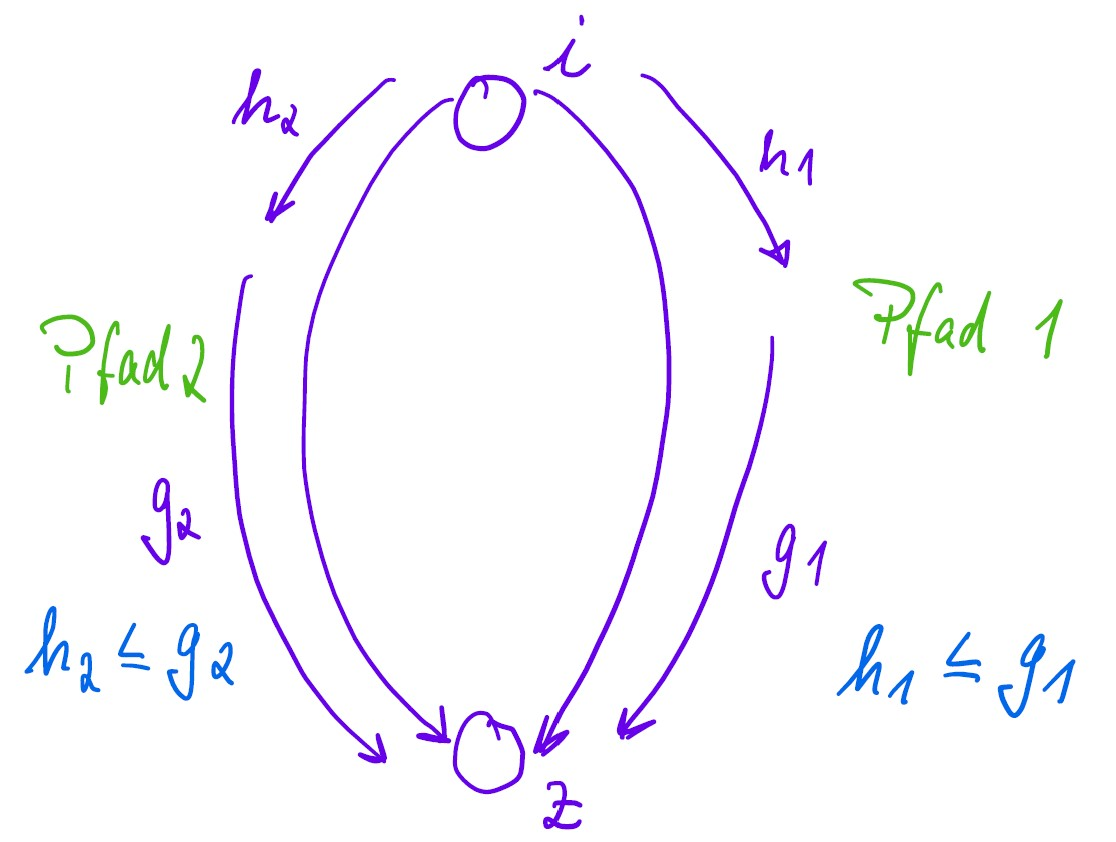
\includegraphics[width=8cm]{a_stern_argument_grafik.jpg}
    \end{center}
    \caption{$A^*$-Algorithmus findet immer das Optimum}    
\end{figure}

Je tiefer der Pfad, desto größer wird $f(n) = g(n) + h(n)$, da $g(n)$ überschätzt und $h(n)$ unterschätzt. Also sind die geschätzten Kosten am Anfang immer geringer als die tatsächlichen Kosten am Ende des Pfades. Somit kann ein gefundener Zielpfad nur der Beste sein, denn gäbe es einen noch besseren Pfad, so wäre dessen Schätzung $h$ noch besser gewesen und wir hätten an irgendeinem Punkt in diese Richtung exploriert und somit den suboptimalen Zielpfad nie gefunden.

Falls gilt:
\begin{enumerate}
    \item $h_1$ und $h_2$ sind zulässig und
    \item $\forall n: h_1(n) \leq h_2(n)$,
\end{enumerate}

dann \textit{exploriert} $A^*$ mit $h_2$ \textit{weniger Knoten} als mit $h_1$; $h_2$ hat dann \textit{mehr Information} als $h_1$.

\subsubsection{Zulässige Schätzfunktionen}
% einfach abtippeln
\begin{itemize}
    \item $\forall n: h(n) = 0 \Rightarrow$ \\ $A*$ entartet zu Breitensuche falls $\forall n: g(n) > 0$.
    \item Es kann \textit{keine zulässige} Schätzfunktion geben, die \textit{Tiefensuche} realisiert \\ (denn DF findet nicht immer das Optimum).
    \item $\forall n: h(n) = h^*(n) \Rightarrow$ \\ \textit{perfekte Heuristik}, aber schwer zu bekommen$\dots$
    \item Bei \textit{endlichen Suchräumen} wird jede Schätzfunktion zulässig durch Division mit einer hinreichend großen Zahl $n$ (z.B. mit $n :=$ \# Knoten im Suchbaum)
    \begin{itemize}
        \item es sollte möglichst gelten $n \approx 1$ \\ (um eine möglichst gute Schätzung $h$ von $h^*$ zu bekommen)
        \item wie geeignetes $n$ finden und \\ was wird die so gewonnene Schätzfunktion taugen? $\rightarrow$ auch wenn sie schlecht ist, ist sie immer noch besser als eine Unzulässige.
    \end{itemize}
\end{itemize}

\subsection{Branch \& Bound}

\textbf{Wurzelpfad:}
\[ \langle n_0, \dots, n_k \rangle \]

vom Startknoten $n_0$ zum Knoten $n_k$ und

\[ c(n_i \rightarrow n_{i+1}) := \text{ Kosten für die Kante } n_i \rightarrow n_{i+1} \]

setzen:

\[ g(n_k) := \sum^{k-1}_{i=0} c(n_i \rightarrow n_{i+1}) \]

Setzt man außerdem
\[ \forall n: h(n) = 0 \]

so wird aus dem $A^*$-Algorithmus die Suchprozedur \textit{Branch \& Bound}. Das heißt es nicht Breitensuche, denn wir explorieren immer den Weg, der in Summe die wenigsten Kosten $g(n)$ hat.

\subsection{Der $A^*$-Algorithmus auf Graphen}

Was ist neu im Vergleich zum normalen $A^*$-Algorithmus?

\begin{enumerate}
    \item Initialisiere $L$ (die \textit{open list}) mit dem Startknoten $s$ für das Problem: $L := \{s\}$.
    \item \color{red} Initialisiere die \textit{closed list} $C$ mit $\emptyset$ und erzeuge einen Explorationsgraphen $G$, der nur $s$ enthält. \color{black}
    \item Ist $L$ leer, so melde einen Fehlschlag.
    \item Andernfalls wähle denjenigen Knoten $n$ aus $L$, für den 
    \[ f(n) = g(n) + h(n) \]
    \textit{minimal} ist \color{red} (dabei bezeichne $g(n)$ die Kosten des günstigsten Pfads vom Startknoten $s$ zu $n$, der bis jetzt gefunden wurde), \\
    entferne $n$ aus $L$ und trage $n$ in $C$ ein. \color{black}
    \item Stellt $n$ einen Zielknoten dar, so melde Erfolg und liefere den Pfad vom Startknoten zu $n$. \textcolor{gray}{Man verfolgt die in $G$ vorhandenen Elternzeiger von $n$ nach $s$ und liefert den Pfad zurück.}
    \item \color{red} Andernfalls expandiere $n$ durch Generieren derjenigen seiner Nachfolger die nicht schon Vorgänger von $n$ in $G$ sind und \\ installiere die Knoten aus der so generierten Menge $M$ als Kinder von $n$ in $G$ (Nachfolgeknoten).
    \item Etabliere in $G$ für alle neuen Knoten aus $M$ (also solche, die nicht schon in $L$ oder $C$ enthalten sind), einen Elternzeiger auf $n$ und füge die neuen Knoten aus $M$ in die Liste $L$ ein.
    \item Entscheide für jeden alten Knoten $m$ aus $M$, ob sein Elternzeiger auf $n$ geändert werden muss, weil der aktuell betrachtete Wurzelpfad von $m$ (mit dem Vater $n$) billiger als der zum alten Elternzeiger von $m$ gehörende Vater ist (Kostenkorrektur). \\ Verfahre entsprechend für die Nachkommen derjenigen alten Knoten aus $m$, die schon in $C$ lagen und gerade eine Kostenkorrektur erfahren haben (rekursive Propagierung der Kostenkorrektur).
    \item Weiter mit Schritt $3$!
\end{enumerate}

Anmerkungen zum Algorithmus:

\begin{itemize}
    \item Der Algorithmus entwickelt in $G$ eine Graphen-Repräsentation ($\rightarrow$ Explorationsgraph)
    \item $G$ enthält einen ausgezeichneten Untergraphen $T$, den sogenannten \textit{Explorationsbaum}
    \item $T$ enthält die gleichen Knoten wie $G$ und ist durch die Elternzeiger aus Schritt $8$ definiert.
    \item $G$ enthält also alle soweit entdeckten Pfade von $s$ zu einem beliebigen Knoten $n \in L \cup C$, wobei jeweils einer dieser Pfade (nämlich genau der mit den geringsten akkumulierten $g$-Kosten) durch die Elternzeiger in $G$ ausgezeichnet wird.
    \item Wendet man diesen Algorithmus auf einen Baum an, so kann man sich natürlich die closed list $C$ und die Verwaltung der Elternzeiger sparen.
\end{itemize}

\begin{lemma}
    Der $A^*$-Algorithmus auf Graphen terminiert für endliche Graphen.
\end{lemma}

\begin{lemma}
    Wenn es überhaupt eine erreichbare Lösung gibt,
    so existiert auf der Open-List $L$ zu jedem Zeitpunkt, bevor der $A^*$-Algorithmus terminiert, ein Knoten $n'$, der sich
    \begin{enumerate}
        \item auf einem optimalen Pfad vom Startknoten $s$ zu einem besten Zielknoten befindet und für den gilt:
        \item $f(n') \leq f^*(s)$
    \end{enumerate}
\end{lemma}

\begin{corollary}
    Falls es einen Pfad vom Startknoten $s$ zu einem Zielknoten gibt, so terminiert der $A^*$-Algorithmus (auch für unendliche Graphen).
\end{corollary}

\begin{corollary}
    Existiert überhaupt eine (erreichbare) Lösung so wird jeder Knoten $n$ auf $L$, für den
    \[ f(n) < f^*(s) \]
    gilt schließlich zur Expansion durch den $A^*$-Algorithmus ausgewählt.
\end{corollary}

\begin{corollary}
    Wenn überhaupt eine (von $s$ erreichbare) Lösung existiert so gilt für jeden von $A^*$ zur Expansion ausgewählten Knoten $n$:
    \[ f(n) \leq f^*(s) \]
\end{corollary}

\begin{definition}
    Eine heuristische Funktion $h$ erfüllt die sogenannte \textit{Monotoniebeschränkung}, wenn für jede Kante $n_i \rightarrow n_j$ mit Kosten $c(n_i \rightarrow n_j)$ des Suchraums
    \[ h(n_i) - h(n_j) \leq c(n_i \rightarrow n_j)\]
    (und außerdem $h(t) = 0$ für alle Zielknoten $t$ gilt.)

    $\Rightarrow$ Je näher wir ans Ziel kommen, desto geringer wird die geschätzte Entfernung zum Ziel. Aber die Differenz der beiden Abschätzungen ist geringer als die Kosten der Modifikation.
\end{definition}

\begin{lemma}
    Erfüllt $h$ die Monotoniebeschränkung, so ist $h$ schon zulässig.
\end{lemma}

\begin{lemma}
    Erfüllt $h$ die Monotoniebeschränkung, so ist $f$ auf Wurzelpfaden monoton steigend, d.h. für jede Kante $n_i \rightarrow n_j$ des Suchraums gilt: 
    \[ f(n_i) \leq f(n_j) \]
\end{lemma}

\begin{theorem}
    Erfüllt die Schätzfunktion $h$ die Monotoniebeschränkung, dann hat der $A^*$-Algorithmus immer schon einen optimalen Pfad für jeden Knoten $n$ gefunden, den er zur Expansion auswählt (es gilt dann also $g(n) = g^*(n)$).

    Also muss der $A^*$-Algorithmus weder Kosten noch irgendwelche Elternzeiger in $G$ aktualisieren.
\end{theorem}

\begin{theorem}
    Erfüllt $h$ die Monotoniebeschränkung, so ist die Folge der $f$-Schätzwerte zu den Knoten, die vom $A^*$-Algorithmus während der Suche der Reihe nach expandiert werden, monoton steigend.
\end{theorem}

\subsection{Iterative Deepening $A^*$}
Wir legen eine maximale Suchtiefe $c$ fest, die wir immer dann erhöhen, wenn die Open-List leer ist. Wir nehmen immer nur Knoten mit $f(n) \leq c$ in die Open-List auf, wodurch diese klein gehalten wird.

\begin{description}
    \item[Speicherbedarf] $\mathcal O(d)$.
    \item[Expandiert] genau die gleichen Knoten wie $A^*$.
    \item[Optimale Lösung] wird wie bei $A^*$ immer gefunden (wenn diese erreichbar und $h$ zulässig ist).
\end{description}


\section{Glaube und Wissen}

\subsection{Lernfragen}
\begin{description}
    \item[Was ist Wissen?]
    \item[Die Trinität von Glaube, Rechtfertigung und Wahrheit]
    \item[Buridan-Sätze]
    \item[Gettier-Beispiele]
    \item[Eine vierte Bedingung]
\end{description}

\subsection{Wissende Agenten}
$\dots$ haben eine eigene Datenbank, die ihre Beliefs enthält. Sie glauben Sätze, die mittels ihrer eigenen Ableitungsregeln von ihrer Datenbank ableitbar sind.

Modaloperator $B$ (Belief) hat zwei Operanden:

\begin{enumerate}
    \item Bezeichner $\alpha$ für einen Agenten
    \item Satz $\phi$
\end{enumerate}

Beliefs stellen selbst Sätze dar: $B_{\alpha}(\phi)$

Zusätzlicher Modaloperator $K$ (Knowledge) vom gleichen Typ:
\[ K_{\alpha}(\phi) := B_{\alpha}(\phi) \land \phi \rightarrow \text{ muss geglaubt werden \textit{und} wahr sein} \]

Die Menge der Agenten erweitern den Interpretationsbereich: Die Agenten haben alle einen eigenen Interpretationsbereich, zusammen ergeben diese den gesamten Interpretationsbereich.

Jeder Agent $\alpha$ hat eine Menge Grundbeliefs $\Delta_{\alpha}$ und eine Menge $\rho_{\alpha}$ von Ableitungsregeln (mit zugehöriger Ableitungsrelation).

Die Theorie ($\tau$) eines Agenten ist die Menge aller Sätze, welche er mit seinen Ableitungsregeln aus seinen Grundbeliefs ableiten kann. Die Theorie eines Agenten ist nicht zwingend abgeschlossen bzgl. der logischen Konsequenz, sondern nur unter den Ableitungsregeln des Agenten. Ein Agent glaubt einen Satz gdw. dieser in seiner Theorie enthalten ist.

\textbf{Semantic Attachment} bedeutet, dass wir mit neuen Beobachtungen bzw. Aussagen aus unserer Welt wiederum neue Aussagen schließen und in unser Beliefsystem aufnehmen können.

Verschachtelte Beliefs sind möglich: $B_{\alpha}(B_{\beta}(\phi)) \rightarrow$ Agent $\alpha$ glaubt, dass Agent $\beta$ an den Sachverhalt $\phi$ glaubt. So kann jede Theorie eines Agenten beliebige Beliefs enthalten.

\subsection{Mögliche Welten}
Zu jedem Agenten gehört eine mögliche Welt (bzw. Weltsicht). Ein Agent glaubt einen Satz relativ zu seiner Welt $W$, wenn der Satz in jeder Welt gilt, die von $W$ erreichbar ist. Alternative Konzeptualisierung von Wissen ist über mögliche Welten $w_0, w_1, \ldots, w_i \in W$ möglich.

Spielen eine Schlüsselrolle bei der Zuordnung von Semantik, falls Sätze den Modaloperator $K$ enthalten. wff's sind somit nicht mehr absolut (also in jeder Welt uneingeschränkt), sondern in bestimmten Welten $w$ wahr. Wir interpretieren also abhängig von der entsprechenden Welt.

\begin{definition}Zugänglichkeitsrelation $k$
    \[ k \in A \times W \times W \]
    (A eine Menge von Agenten und $W$ Menge der möglichen Welten)
    
    gilt

    \[ k(\alpha, w_i, w_j) \]

    so heißt

    \begin{enumerate}
        \item für den Agenten $\alpha$
        \item $w_j$ zugänglich von $w_i$
    \end{enumerate}
\end{definition}

Wenn wir zu einer \textbf{K}-Aussage nicht ausdrücklich die Welt nennen, beziehen wir uns damit auf die aktuelle Welt $w_0$.

Somit ist ein Atom genau dann Wissen eines Agenten bezüglich einer bestimmten Welt $w_i$, wenn für alle vom Agenten von $w_i$ aus erreichbaren Welten gilt, dass dieses Atom dort gilt. So kann, genau wie bei Beliefs, auch wieder verschachtelt werden.

Die mögliche Welten Semantik impliziert logische Allwissenheit der Agenten, eine Zugangsrelation für Glaube (Beliefs) ist daher nicht sinnvoll.

\subsection{Axiomatisierung von Wissen}

Axiom $\estimates$ wahr angenommener Grundsatz. Also sind unsere Axiome die jeweiligen Beliefs der einzelnen Agenten.

Notwendige Eigenschaften von $K$ und $B$ (damit sie die übliche Vorstellung von Wissen / Glaube widerspiegeln)

\begin{enumerate}
    \item Agent kann mit seinem Wissen schlussfolgern
    \item Agent kann nichts wissen, was falsch ist (Wissensaxiom)
    \begin{enumerate}
        \item Setzt Reflexivität von $K$ voraus. Für alle Welten $w$ gilt, dass $w$ von $w$ zugänglich ist.
        \item Ein Agent kann auch keine Widersprüche wissen (z.B. $P \land \lnot P$)
    \end{enumerate}
    \item $k$ ist \textbf{seriell} $\leftrightarrow$ für alle Agenten von einer beliebigen Welt $w_1$ aus mindestens eine weitere Welt $w_2$ zugänglich ist. (Die Zugangsrelation hat also keine Sackgassen.)
    \item Falls $k$ transitiv (wie üblich definiert) ist, sind Agenten zur positiven Introspektion in der Lage. Das heißt, sie wissen, dass sie selbst etwas wissen (geschachteltes Wissen über sich selbst)
    \item Negative Introspektionsfähigkeit: Wenn man $\phi$ nicht weiß, dann weiß man, dass man es nicht weiß. (falls $k$ euklidisch)
    \begin{enumerate}
        \item $k$ ist \textbf{euklidisch} wenn man von $w_1$ sowohl zu $w_2$ als auch zu $w_3$ kommt, dann kommt man auch von $w_2$ zu $w_3$.
        \item $k$ ist \textbf{symmetrisch}: Man kommt von $w_1$ zu $w_2$ gdw. man von $w_2$ zu $w_1$ kommt. Daraus folgt das Brouwer Axiom: doppelt verneintes Wissen führt dazu, dass der Satz wahr ist.
    \end{enumerate}
    \item Epistemische Notwendigkeit: wenn wir aus Nichts $\phi$ ableiten können, dann wissen wir $\phi$.
\end{enumerate}

Die Axiome $1$ bis $6$ machen einen Agenten logisch allwissend, falls der Modus Ponendo Ponens (Implikationsregel + Sachverhalt tritt ein) die einzige Ableitungsregel ist. Falls nur einzelne Axiome gelten, ergeben sich verschiedene epistemische Modallogiken.
Distributivität über Konjunktion funktioniert, über Disjunktion nur bedingt. Rechenregeln existieren.

\subsection{Gettier-Beispiele}
Es ist möglich einen gerechtfertigen, wahren Glauben zu besitzen und dennoch nicht zu wissen, was man glaubt.

Kernidee eines Gettier-Beispiels: Aus dem richtigen Grund Recht haben, ohne dass die Gründe gelten.

\begin{example}
    Ein Kollege kommt aus der Mittagspause zurück und fragt nach der Uhrzeit. Wir schauen gemeinsam auf meine Funkuhr: $14.14$

    Danach ist der Glaube, dass es $14.14$ ist, gerechtfertigt. 

    Was gilt aber, wenn wir genau um $14.14$ auf die Uhr schauen, die Uhr aber in der Nacht zuvor um $2.14$ stehengeblieben ist?
\end{example}

Niemand weiß, wann ein Glaube durch ein Widerlegungselement bedroht ist. (Daher kann man nicht fordern, dass wir nur korrekt begründete Glauben als Wissen einstufen.)

\subsection{Eigenschaften von Beliefs}
\begin{itemize}
    \item Ein Agent kann auch nur EINEN von zwei äquivalenten Sätzen glauben (Bsp. Venus und Abendstern). Nur weil er an einen Satz glaubt, heißt das nicht, dass er an alle äquivalenten Sätze auch glaubt. $\rightarrow$ das nennt man referentiell opake Kontexte (im Gegensatz zu referentiell transparenten Kontexten. Dort gilt: Sind $A$ und $B$ äquivalent, dann folgt aus dem Glauben an $A$ auch der Glaube an $B$).
    \item Können verschachtelt werden (beliebig tief)
    \item Man kann auch Falsches glauben, man kann aber nichts Falsches wissen.
    \item Ein wahrer Glaube muss aber vom Agenten nicht unbedingt als Wissen eingestuft werden. (Gettier-Beispiele)
    \item Wichtige Axiome für Glaube:
    \begin{enumerate}
        \item Widersprüche werden nicht geglaubt
        \item Positive Introspektionsfähigkeit: wir glauben etwas, deshalb glauben wir auch, dass wir es glauben (negative Introspektion eventuell problematisch)
        \item Agenten wissen, was sie glauben
        \item (optional: Agenten glauben alles, was ihre Kollegen glauben)
    \end{enumerate}
\end{itemize}

\subsection{Monotonie vs. Nicht-Monotonie}

\[ \text{Cn}(A) := \{\phi | A \rightarrow \phi \} \]

ist die syntaktische Konsequenz. $\text{Cn}(A)$ ist die deduktive Hülle von $A$, also alles, was aus $A$ ableitbar ist. (alternative: $\text{Cn}'$ für die direkte Folgerbarkeit)

\begin{description}
    \item[Klassisches Folgern] Ableiten über eine Reihe von Formeln
    \item[Monotonie] Wenn zur alten Wissensbasis $A$ neue Informationen dazukommen, so bleiben alle alten Ableitungen aus $A$ immer noch bestehen, sind also immer noch ableitbar.
    \item[Idempotenz] $\text{Cn}(A) = \text{Cn}(\text{Cn}(A)) \rightarrow $ Die deduktive Hülle der deduktiven Hülle ist immer noch die deduktive Hülle.
\end{description}

Monotonie und Idempotenz sind für den klassischen Folgerungsbegriff charakteristisch!

Für eine nicht monotone Logik gilt die Monotonieeigenschaft nicht. Da unser Wissen über die Welt unvollständig ist, müssen wir (plausible) Annahmen treffen (Beliefs), die sich aber später als falsch herausstellen können. Deshalb gilt:

\par
\textbf{Temporale Nicht-Monotonie:} Dinge, die wir zu einem früheren Zeitpunkt glauben, glauben wir (aufgrund neuer Erkenntnisse) zu einem späteren Zeitpunkt nicht mehr zwingend. $\rightarrow$ Belief Revision notwendig!

Beispiel für NM-Schließen: Kann der Strauß Tweety fliegen?

\subsection{Belief Revision}

Wie eine widerlegte Theorie, die aufgrund neuer Erkenntnisse angepasst werden muss.

Gegeben: ein epistemischer Zustand $A$ und eine Proposition $x$. Man knan zwei Revisionsoperationen unterscheiden:

\begin{enumerate}
    \item Expansion $A + x$: Verändere $A$ minimal, sodass $x$ enthalten und $A$ konsistent ist.
    \item Kontraktion $A - x$: Verändere $A$ minimal, sodass $x$ nicht enthalten ist.
\end{enumerate}

Damit ist das genaue Vorgehen der Belief Revision noch vollkommen unklar, denn es ergeben sich einige nicht-triviale Fragen:

\begin{itemize}
    \item Was sind vernünftige Revisionsoperatoren?
    \item Wie kann man "minimale Änderung" formal fassen?
\end{itemize}

Gegeben ist ein Artefakt, beschrieben durch das logische Modell. Also:

\begin{enumerate}
    \item Eine Menge von Formeln, die das korrekte Verhalten beschreiben.
    \item Eine Menge von Normalitätsannahmen, die das Funktionen von Komponenten postuliert.
\end{enumerate}

Steht das beobachtete Verhalten des Systems im Widerspruch zum Verhalten, welches vom Modell postuliert wurde, so besteht Diagnosebedarf!

Ansatz der \textbf{konsistenzbasierten Diagnose:} egal wie, Hauptsache die Welt bzw. das System ist danach wieder konsistent. Dabei ist die Diagnose meist nicht eindeutig. Wir suchen kleine Teilmengen, die (vermutlich) den Widerspruch verantworten.

Hilfreich ist dabei neben einem Wohlverhaltensmodell ein Fehlverhaltensmodell, das uns sofort sagt, was (vermutlich) getan werden muss, falls eine bestimmte Komponente nicht funktioniert. (Beispiel: kaputtes Auto oder Krankheitssymptome)

\subsection{Formen der Inferenz}

\begin{enumerate}
    \item \textbf{Deduktion} $a, a\rightarrow b \Rightarrow b$
    \begin{enumerate}
        \item Wir kennen die Regeln $a\rightarrow b$ und beobachten $a$, schlussfolgern also $b$.
        \item Wir schließen aus wahren Sachverhalten andere wahre Sachverhalte.
    \end{enumerate}
    \item \textbf{Induktion} $a, b\rightarrow a \Rightarrow a\rightarrow b$
    \begin{enumerate}
        \item Wir beobachten $a$ und $b$ gemeinsam und schließen daraus, dass $a\rightarrow b$ gelten muss.
        \item Wir Generalisieren durch Beobachten. Kausalität ist daher nicht zwingend gegeben und kann falsch sein!
    \end{enumerate}
    \item \textbf{Abduktion} $a \rightarrow b, b \Rightarrow a$
    \begin{enumerate}
        \item Wir wissen, dass aus $a$ $b$ folgt und beobachten $b$. Deshalb schließen wir $a$.
        \item Kann natürlich falsch sein. \textit{Beispiel:} $a\estimates$"Es regnet", $b\estimates$"die Straße ist nass"
        \item Abduktion findet vor Gericht statt, die beste Erklärung gewinnt!
        \item Abduktion ist nicht-monotone Erklärungsinferenz: Von den Wirkungen zu den plausiblen Ursachen!
    \end{enumerate}
\end{enumerate}

\subsection{Default-Logik}

Wir führen zusätzlich nicht-logische Inferenzregeln ein: Regeln, die fast immer wahr sind, bis auf Ausnahmen.

"Vögel fliegen typischerweise" ist eine solche Aussage. Schließen ist somit nicht mehr monoton, denn ich darf diese Ableitung so lange normal durchführen, bis sie zu einem Widerspruch führen würde. Ich prüfe also erst auf Widersprüche und leite dann ab (nicht mehr monoton und außerdem deutlich aufwendiger)!

$\text{flies}(x)$ ist hierbei der default.

Ausnahmen werden durch einfache Implikationen dargestellt: $\text{penguin}(x) \rightarrow \text{not-flies}(x)$.

\par \textbf{Eigenschaften des Default-Schließens}
\begin{itemize}
    \item Nicht-Monotonie
    \item Nicht-Determinismus $\rightarrow$ verschiedene Regeln können sich widersprechende Dinge schließen (Beispiel: Heimatstadt Ehepaar, Nixon)
    \item Default-Regeln dienen zur Ergänzung(!) von unvollständigen Theorien
\end{itemize}

Default-Regeln bestehen aus Voraussetzung, Begründung und Konsequenz. Sie heißen abgeschlossen, wenn sie keine freien Variablen enthalten.

Ein Paar $(D, W)$ ist eine Default-Theorie ($D$=Defaults, $W$=Menge an PL1-Logiken). Die Defaults werden dann auch Default-Extensionen genannt. Sie sollten alle Fakten aus $W$ enthalten (die für den Default notwendig sind) und deduktiv abgeschlossen sein, also $E = \text{Cn}(E)$.

\subsection{Theorie-Transformation}

Alternative zu Default-Logiken, die Normalitätsannahmen verwendet.

\begin{itemize}
    \item \textit{Beispiel}: Normale vs. Abnormale Vögel: $\text{bird}(x) \land \text{normal}(x) \rightarrow \text{flies}(x)$ 
    \item Normale Vögel können fliegen, abnormale Vögel können nicht fliegen.
    \item \textit{aber}: normale Straußen können nicht fliegen! (abnormale in einem Flugzeug vielleicht schon $\dots$)
    \item Also sind Dinge nicht generell abnormal, sondern in Bezug auf ein bestimmtest Prädikat (\textit{Beispiel}: Vogel, Fliegen, etc.)
\end{itemize}

\textbf{Problem der temporalen Projektion:} Welche Eigenschaften gelten, nachdem bestimmte Ereignisse stattgefunden haben? Vor allem solche, die nicht syntaktische oder logische Konsequenz sind?

\textbf{Das Frame-Problem:} riesige Anzahl an Axiomen wäre nötig. Aber: McCarthy's Formulierung besagt, dass alle "normalen" Fakten nach "normalen" Ereignissen gelten. So muss das "abnormal"-Prädikat nicht so oft verwendet werden. % TODO wer ist McCarthy??

\subsection{Poole-Erweiterungen}

Sei $T$ eine Menge an Sätzen, die nie zurückgenommen werden müssen und $A$ eine Menge an Annahmen, die wir dementsprechend als revidierbar betrachten.

Das Paar $(T,A)$ ist eine nicht monotone Theorie mit Basistheorie $T$.

Eine \textbf{Poole-Erweiterung} einer nicht-monotonen Theorie $(T,A)$ ist eine maximale Teilmenge $E$ von $A$, die konsistent mit $T$ ist. (also der Teil der Annahmen, der den Grundsätzen nicht widerspricht)

Auch Poole-Erweiterungen sind nicht immer eindeutig! Siehe Nixon-Beispiel: Es sind zwei Poole-Erweiterungen möglich (er ist religieus normal oder politisch normal) die sich gegenseitig widersprechen, einzeln aber nicht zuu einem Widerspruch mit $T$ führen.

Seit $(T,A)$ eine nicht-monotone Theorie. Dann heißt ein Satz $p$ \textit{skeptische Konsequenz} von $(T,A)$, wenn er in jeder und \textit{leichtgläubige Konsequenz}, wenn er in mindestens einer Poole-Erweiterung $E$ von $T$ Konsequenz ist.

Im Zweifel entscheidet man sich bei widersprüchlichen leichtgläubigen Konsequenzen für die kürzere inferentielle Distanz, also für den kürzeren "Ableitungspfad".

\subsection{Skeptische und leichtgläubige Konsequenzten}

Wie berechnet man, ob eine Anfrage $q$ leichtgläubige bzw. skeptische Konsequenz von $(T,A)$ ist?

\par $\rightarrow$ Das Überprüfen aller Poole-Erweiterungen ist viel zu teuer und unnötig.

\textit{Lösung:} $S$ ist eine Erklärung für $q$ relativ zu $(T,A)$, wenn gilt:

\begin{enumerate}
    \item $S$ ist Teilmenge von $A$.
    \item $S$ ist konsistent mit $T$ (also kein Widerspruch).
    \item Aus $T \cup S \vdash q$ (bzw. lässt sich $q$ schließen)
    \item $S$ ist eine minimale Menge mit dieser Eigenschaft.
\end{enumerate}

Es gibt (vergleichsweise) effiziente Algorithmus zur Berechnung von Erklärungen.

\begin{example} Nixon-Diamant\\
    "Nixon ist Pazifist"
\end{example}


% TODO Heuristische Suche ergänzen

\pagebreak

\section{Prüfungsfragen}
\begin{enumerate}
    \item Was ist KI?
    \item Was ist Suche?
    \begin{enumerate}
        \item Suchproblem modellieren
        \item KEIN Min-Max wird abgefragt!
        \item Beispiel $\rightarrow$ Navigationssystem (Lösung: nicht der kürzeste Weg, sondern ein Pfad.)
        \begin{itemize}
            \item Knoten: Orte in Stadt
            \item Kanten: Aktionen von Ort zu Ort
            \item $\rightarrow$ generiert von Startknoten aus.
            \item Suchverfahren: Breitensuche, Tiefensuche, Heuristik
            \item Breitensuche:
            \begin{enumerate}
                \item Kosten: Zeit / Entfernung $\infty > Kosten > 0$
                \item Handlungsmöglichkeiten $< \infty$
            \end{enumerate}
            Heuristik:
            \begin{itemize}
                \item effizienter: $\rightarrow$ Zeit und Speicheraufwand
                \item Bspw.: Luftlinie als Heuristik
                \item Eine Heuristik ist zulässig, wenn
                \begin{itemize}
                    \item[$\rightarrow$] optimale Lösung $\rightarrow$ 
                    \item[$\rightarrow$] monotoniebeschränkung $\rightarrow$ Warum führt die monotoniebeschränkung dazu, dass man nicht zweimal den gleichen Weg findet? 
                \end{itemize}
            \end{itemize}
            \item A-Algorithmus
            \begin{itemize}
                \item[$\rightarrow$] open-list zu exp. Knoten $f(n) = h(n) + g(n)$ 
                \item[$\rightarrow$] closed-list (braucht man eigentlich nicht, da die Heuristik monotoniebeschränkt ist)
            \end{itemize}
        \end{itemize}
    \end{enumerate}
    \item Logik
    \begin{itemize}
        \item Resolution ($\rightarrow$ siehe oben)
        \item Logische Konsequenz
        \item Kalkül
        \begin{itemize}
            \item Sprache (Symbole und syntaktische Regeln) $\Gamma_\alpha= \{P \; |\; \delta_\alpha \vdash_\alpha P\}$
            \item Ableitungsregeln
            \item Axiome
        \end{itemize}
        \item Wissen
        \begin{itemize}
            \item Trinität: Glaube, Rechtfertigung, Wahrheit (Wahrheitswerttabelle aufstellen und ausführlich erklären)
            \item Gettier-Beispiele, Buridan-Sätze (kann man nicht mit dieser Trinität aufstellen, weil es einen Selbstbezug gibt)
        \end{itemize}
    \end{itemize}
    \item Mögliche Welten und Agenten
    \begin{itemize}
        \item semantic attachment: Wenn wir neue Aussage aus unserer Welt bkeommen, die noch nicht in unseren Beliefs sind, dannn können wir die nutzen um neue Aussagen in usner Beliefsystem aufzunehmen.
        \begin{align*}
            B_\alpha(\Phi_1) \lor \Psi_1 \\
            \vdots \\
            B_\alpha(\Phi_n) \lor \Psi_n \\
            \lnot B_\alpha(\Psi_{n+1}) \lor \Psi_{n+1} \\
            \phi_1 \land \phi_2 \land \dots \land \psi_n \vdash \phi_{n+1} \\
            \hline
            \psi_1 \lor \psi_2 \lor \dots \lor \psi_{n+1}
        \end{align*}
        \begin{align*}
            B_\alpha(\phi_1) \lor \text{ kein Vogel} \\
            \lnot B_\alpha(\phi_2) \lor \text{ kein Säugetier} \\
            \text{kann fliegen } \vdash \text{ hat Flügel}
        \end{align*}
    \end{itemize}
    \item Nicht-Monotonie (wird er nicht so tief fragen, er geht eher auf Objektzentrierte Wissensrepräsentation ein)
    \begin{itemize}
        \item Wenn wir einmal etwas festgelegt haben, können wir keine Widersprüche glauben. 
        \item $\rightarrow$ Poole-Erweiterung (sind Defaults) $\hookrightarrow$ Wir behalten die Maximale Menge an Normalitäten und ersetzen nur mit einer minimalen Menge an Abnormalitäten. Wir versuchen möglichst viel von unserem Wissen zu behalten und möglichst wenig wegzuwerfen.
    \end{itemize}
    \item Objektzentrierte Wissensrepräsentation
    \item Ontologie (legt er fokus), A-Box, T-Box erklären können, Warum ist die T-Box gerade die Ontologie?
    \item Die Objekte sind Anreicherung des Wissensgraphen mit konkreten Beispielen
    \item Probleme aus der Objektzentrierten Wissensrepräsentation werden durch probabilistisches Schließen gelöst. Also sollte man erklären können, wie die Probleme gelöst werden.
\end{enumerate}

\end{document}
 